\documentclass[tikz,border=6pt]{standalone}
\usepackage{tikz}
\usepackage{pgfplots}
\pgfplotsset{compat=1.18}
\begin{document}
% Data from paper/CAL/build/extract_cosim_heatmap.py (fig4_cosim_data.json).
% Rows: SA size in {16x16, 32x32, 48x48}. Cols: APT config in {off, density-only, precision-only, full}.
% Color = FPS (higher = better). Text overlay = KITTI D1% (lower = better).
% D1 is algorithmic and SA-invariant; FPS responds to both axes.
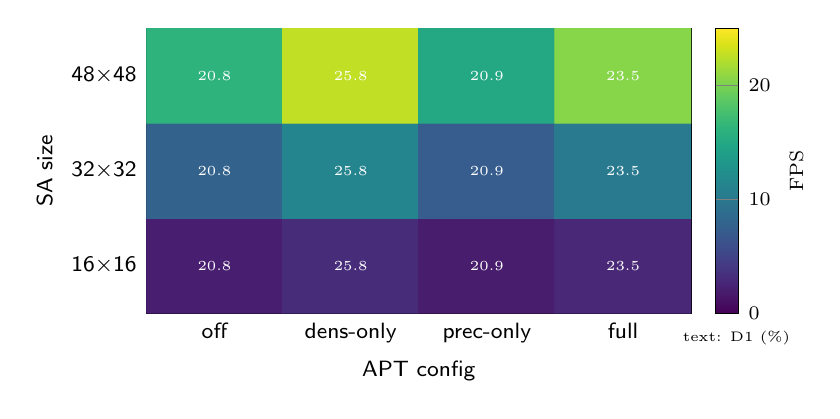
\begin{tikzpicture}
\begin{axis}[
  font=\sffamily\footnotesize,
  width=8.5cm,height=5.2cm,
  view={0}{90},
  colormap/viridis,
  colorbar,
  colorbar style={
    width=3mm,
    ylabel={FPS},
    font=\scriptsize,
  },
  xlabel={APT config},
  ylabel={SA size},
  xtick={0,1,2,3},
  xticklabels={off,dens-only,prec-only,full},
  ytick={0,1,2},
  yticklabels={16$\times$16,32$\times$32,48$\times$48},
  enlargelimits=false,
  point meta min=0,
  point meta max=25,
]
% 3x4 grid: rows = SA size (0..2), cols = APT config (0..3)
% values are FPS; D1% overlaid as node text
\addplot[matrix plot*,mesh/cols=4,point meta=explicit] coordinates {
(0,0) [ 2.06] (1,0) [ 3.07] (2,0) [ 1.91] (3,0) [ 2.75]
(0,1) [ 7.80] (1,1) [11.37] (2,1) [ 7.24] (3,1) [10.21]
(0,2) [16.16] (1,2) [22.71] (2,2) [15.02] (3,2) [20.52]
};
% D1% overlays (invariant along rows)
\node[font=\tiny,white] at (axis cs:0,0) {20.8};
\node[font=\tiny,white] at (axis cs:1,0) {25.8};
\node[font=\tiny,white] at (axis cs:2,0) {20.9};
\node[font=\tiny,white] at (axis cs:3,0) {23.5};
\node[font=\tiny,white] at (axis cs:0,1) {20.8};
\node[font=\tiny,white] at (axis cs:1,1) {25.8};
\node[font=\tiny,white] at (axis cs:2,1) {20.9};
\node[font=\tiny,white] at (axis cs:3,1) {23.5};
\node[font=\tiny,white] at (axis cs:0,2) {20.8};
\node[font=\tiny,white] at (axis cs:1,2) {25.8};
\node[font=\tiny,white] at (axis cs:2,2) {20.9};
\node[font=\tiny,white] at (axis cs:3,2) {23.5};
\end{axis}
\node[font=\tiny,anchor=north east] at (8.3,-0.1) {text: D1 (\%)};
\end{tikzpicture}
\end{document}
